% Modified based on Xiaoming Sun's template
\documentclass{article}
\usepackage{amsmath,amsfonts,amsthm,amssymb}
\usepackage{setspace}
\usepackage{fancyhdr}
\usepackage{lastpage}
\usepackage{extramarks}
\usepackage{chngpage}
\usepackage{soul,color}
\usepackage{graphicx,float,wrapfig}
\usepackage{enumitem}
\usepackage{array} 
\renewcommand{\d}{\mathrm{d}}
\newcommand{\Class}{Pattern Recognition and Machine Learning}

% Homework Specific Information. Change it to your own
\newcommand{\Title}{Homework 5}

% In case you need to adjust margins:
\topmargin=-0.45in      %
\evensidemargin=0in     %
\oddsidemargin=0in      %
\textwidth=6.5in        %
\textheight=9.0in       %
\headsep=0.25in         %

% Setup the header and footer
\pagestyle{fancy}                                                       %
\chead{\Title}  %
\rhead{\firstxmark}                                                     %
\lfoot{\lastxmark}                                                      %
\cfoot{}                                                                %
\rfoot{Page\ \thepage\ of\ \protect\pageref{LastPage}}                          %
\renewcommand\headrulewidth{0.4pt}                                      %
\renewcommand\footrulewidth{0.4pt}                                      %

%%%%%%%%%%%%%%%%%%%%%%%%%%%%%%%%%%%%%%%%%%%%%%%%%%%%%%%%%%%%%
% Some tools
\newcommand{\enterProblemHeader}[1]{\nobreak\extramarks{#1}{#1 continued on next page\ldots}\nobreak%
                                    \nobreak\extramarks{#1 (continued)}{#1 continued on next page\ldots}\nobreak}%
\newcommand{\exitProblemHeader}[1]{\nobreak\extramarks{#1 (continued)}{#1 continued on next page\ldots}\nobreak%
                                   \nobreak\extramarks{#1}{}\nobreak}%

\newcommand{\homeworkProblemName}{}%
\newcounter{homeworkProblemCounter}%
\newenvironment{homeworkProblem}[1][Problem \arabic{homeworkProblemCounter}]%
  {\stepcounter{homeworkProblemCounter}%
   \renewcommand{\homeworkProblemName}{#1}%
   \section*{\homeworkProblemName}%
   \enterProblemHeader{\homeworkProblemName}}%
  {\exitProblemHeader{\homeworkProblemName}}%

\newcommand{\homeworkSectionName}{}%
\newlength{\homeworkSectionLabelLength}{}%
\newenvironment{homeworkSection}[1]%
  {% We put this space here to make sure we're not connected to the above.

   \renewcommand{\homeworkSectionName}{#1}%
   \settowidth{\homeworkSectionLabelLength}{\homeworkSectionName}%
   \addtolength{\homeworkSectionLabelLength}{0.25in}%
   \changetext{}{-\homeworkSectionLabelLength}{}{}{}%
   \subsection*{\homeworkSectionName}%
   \enterProblemHeader{\homeworkProblemName\ [\homeworkSectionName]}}%
  {\enterProblemHeader{\homeworkProblemName}%

   % We put the blank space above in order to make sure this margin
   % change doesn't happen too soon.
   \changetext{}{+\homeworkSectionLabelLength}{}{}{}}%

\newcommand{\Answer}{\ \\\textbf{Answer:} }
\newcommand{\Acknowledgement}[1]{\ \\{\bf Acknowledgement:} #1}

%%%%%%%%%%%%%%%%%%%%%%%%%%%%%%%%%%%%%%%%%%%%%%%%%%%%%%%%%%%%%


%%%%%%%%%%%%%%%%%%%%%%%%%%%%%%%%%%%%%%%%%%%%%%%%%%%%%%%%%%%%%
% Make title
\title{\textmd{\bf \Class: \Title}}
  \date{\textbf{\today}}
\author{\textbf{Qingru Hu \quad 2020012996}}
%%%%%%%%%%%%%%%%%%%%%%%%%%%%%%%%%%%%%%%%%%%%%%%%%%%%%%%%%%%%%

\begin{document}
\begin{spacing}{1.1}
\maketitle \thispagestyle{empty}

%%%%%%%%%%%%%%%%%%%%%%%%%%%%%%%%%%%%%%%%%%%%%%%%%%%%%%%%%%%%%
% Begin edit from here

\begin{homeworkProblem}
% \Answer \\
The posterior distribution of $\omega_i, i=1, 2$ is that:
\begin{align*}
  P(\omega_1 \vert (x, y)) &= \frac{P(x, y \vert \omega_1) P(\omega_1)}{P(x, y)} = C \frac{1}{3\pi} e^{-\frac{x^2 + y^2}{2}} \\
  P(\omega_2 \vert (x, y)) &= \frac{P(x, y \vert \omega_2) P(\omega_2)}{P(x, y)} = C \frac{1}{6\pi} e^{-\frac{(x-2)^2 + (y-2)^2}{2}} \\
\end{align*}
Given that the probability $P(x, y)=1/C$ is a constant, according to the minimum prediction error principle, 
we can have the optimal classifier:
$$f(x,y)= \omega^* =
\begin{cases}
\omega_1& P(\omega_1 \vert (x, y)) > P(\omega_2 \vert (x, y))\\
\omega_2& P(\omega_1 \vert (x, y)) \leq P(\omega_2 \vert (x, y))
\end{cases}$$
Let $P(\omega_1 \vert (x, y)) = P(\omega_2 \vert (x, y))$ and we can get the decision boundary as shown in Fig.\ref{db}:
\begin{align*}
  x+y-2-\frac{1}{2} \ln 2 = 0
\end{align*}
\begin{figure}[htbp]
  \centering
  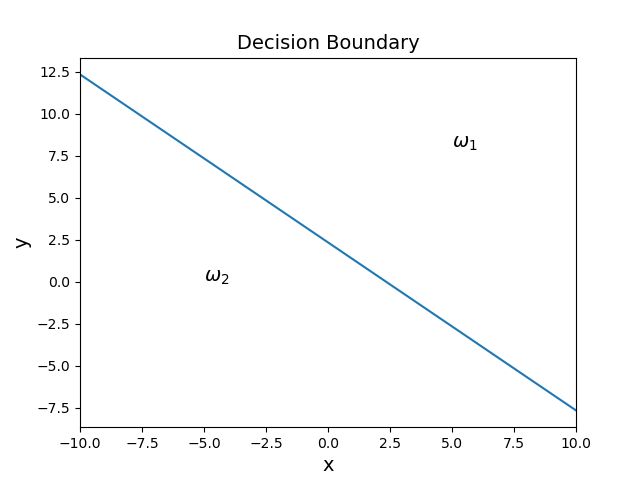
\includegraphics[width=8cm]{db.png}
  \caption{The decision boundary for $(x, y)$}
  \label{db}
\end{figure}
\end{homeworkProblem}

\begin{homeworkProblem}
  If the final classifier outputs $f^*(x)=\omega_1$, the expected cost of $f(x)=\omega_1$ is smaller than or equal to that of $f(x)=\omega_2$:
\begin{align*}
  \int_x \lambda_2 P(\omega_2, x) \d x &\leq \int_x \lambda_1 P(\omega_1, x) \d x \\
  \lambda_2 P(\omega_2, x) &\leq \lambda_1 P(\omega_1, x) \\
  \frac{P(\omega_1, x)}{P(\omega_2, x)} &\geq \frac{\lambda_2}{\lambda_1} \\
  \frac{P(\omega_1\vert x)}{P(\omega_2 \vert x)} &\geq \frac{\lambda_2}{\lambda_1}
\end{align*}
Vice versa, if $\frac{P(\omega_1 \vert x)}{P(\omega_2 \vert x)} \geq \frac{\lambda_2}{\lambda_1}$, then:
\begin{align*}
  \frac{P(\omega_1, x)}{P(\omega_2, x)} &\geq \frac{\lambda_2}{\lambda_1} \\
  \int_x \lambda_2 P(\omega_2, x) \d x &\leq \int_x \lambda_1 P(\omega_1, x) \d x 
\end{align*}
the expected cost of $f(x)=\omega_1$ is smaller than or equal to that of $f(x)=\omega_2$, 
so the final classifier outputs $f^*(x)=\omega_1$.

Specially, when $\lambda_1 = \lambda_2$, this corresponds to our original max-posterior-solution.
\end{homeworkProblem}

\begin{homeworkProblem}
  The hypothesis class is:
\begin{align*}
  \mathcal{H} = \{h(x)=(-1)^{k+\mathbb{I}[a\leq x \leq b]}: k\in\{0, 1\}, a, b\in \mathbb{R}, a\leq b\}
\end{align*}
Since $k$ and $\mathbb{I}[a\leq x \leq b]$ can only have values of 0 or 1, the class labels are $1$ and $-1$.

Suppose we have three points $x_1 < x_2 < x_3$, there are 8 possible labelings and all the possible labelings can be classified by 
a specific function (a specific set of $(k, a, b)$) in $\mathcal{H}$:
\begin{table}[htbp]
  \centering
  \setlength{\tabcolsep}{6mm}{
  \begin{tabular}[pos]{|c|c|c|c|c|}
    \hline
      $x_1$ & $x_2$ & $x_3$ & $k$ & $a, b$ satisfy \\
      \hline
      1 & 1 & 1 & 1 & $a<x_1<x_2<x_3<b$ \\
      \hline
      -1 & 1 & 1 & 1 & $x_1<a<x_2<x_3<b$ \\
      \hline
      1 & -1 & 1 & 0 & $x_1<a<x_2<b<x_3$ \\
      \hline
      1 & 1 & -1 & 1 & $a<x_1<x_2<b<x_3$ \\
      \hline 
      -1 & -1 & 1 & 1 & $x_1<x_2<a<x_3<b$ \\
      \hline
      -1 & 1 & -1 & 1 & $x_1<a<x_2<b<x_3$ \\
      \hline
      1 & -1 & -1 & 1 & $a<x_1<b<x_2<x_3$ \\
      \hline
      -1 & -1 & -1 & 0 & $a<x_1<x_2<x_3<b$ \\
      \hline
  \end{tabular}}
\end{table}

However, for four points $x_1 < x_2 < x_3 < x_4$, the label of $(1, -1, 1, -1)$ can not be classified by any 
function in $\mathcal{H}$. Therefore, the VC dimension of $\mathcal{H}$ is 3.

\end{homeworkProblem}

\begin{homeworkProblem}
\section*{(1)}
I use Parzen window of width $h=2$ to estimate the density function of P(x, y). The the density function 
is shown in Fig.\ref{p_win}.
\begin{figure}[htbp]
  \centering
  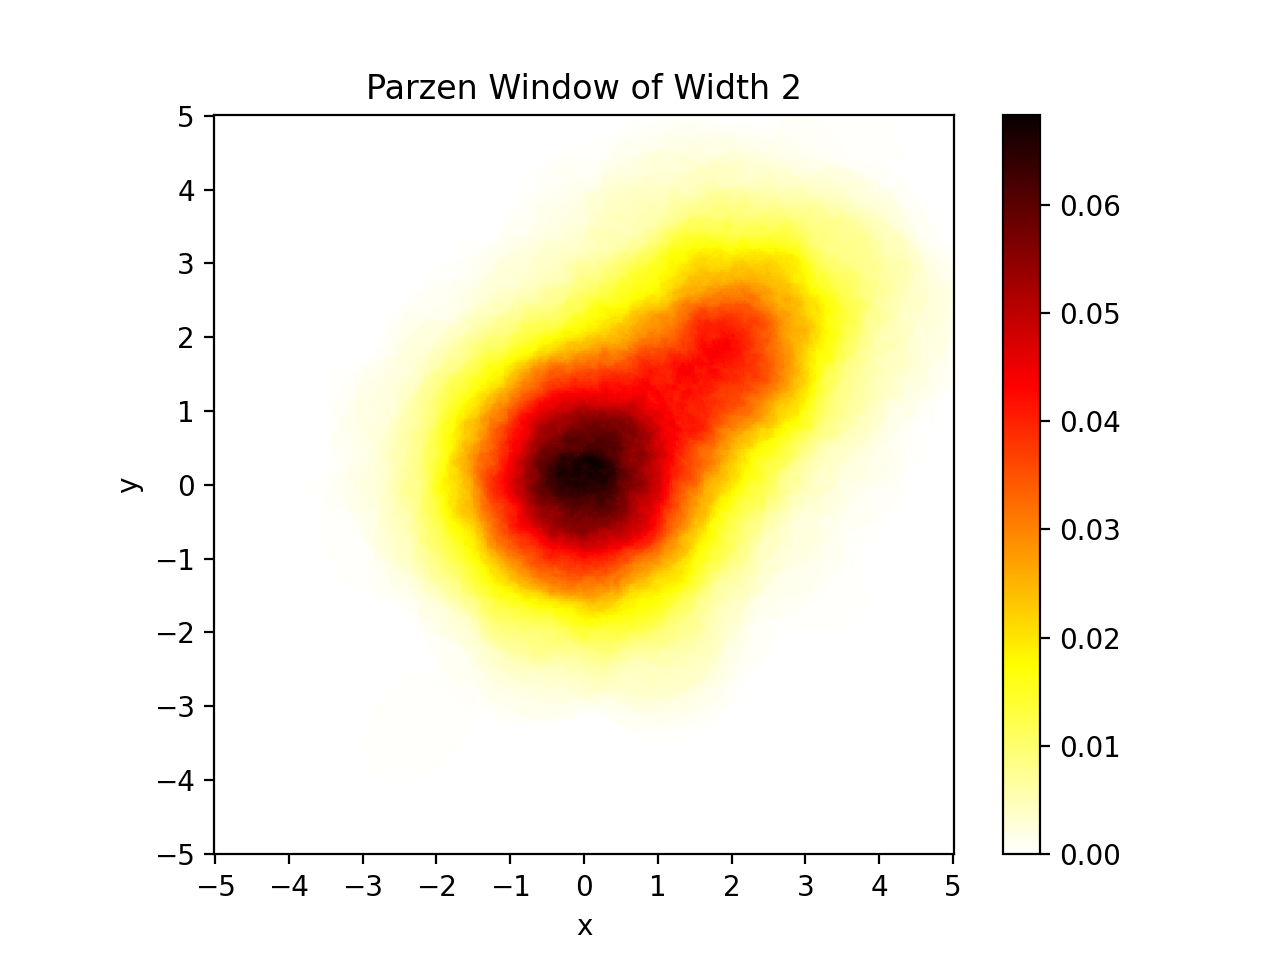
\includegraphics[width=8cm]{p_win.png}
  \caption{The heatmap of desity function from parzen window of width $h=2$}
  \label{p_win}
\end{figure}

\section*{(2)}
Change the window width in $[0.3, 0.5, 1]$ and kernel function in [`Parzen', `Gaussian', `Exp'], 
plot the heatmap, and calculate the mean density error. All the relative information are labelled in figures.
According the mean density error, the kernel function `Gaussian' with window width of $0.5$ is the best composition.
\begin{figure}[htbp]
  \centering
  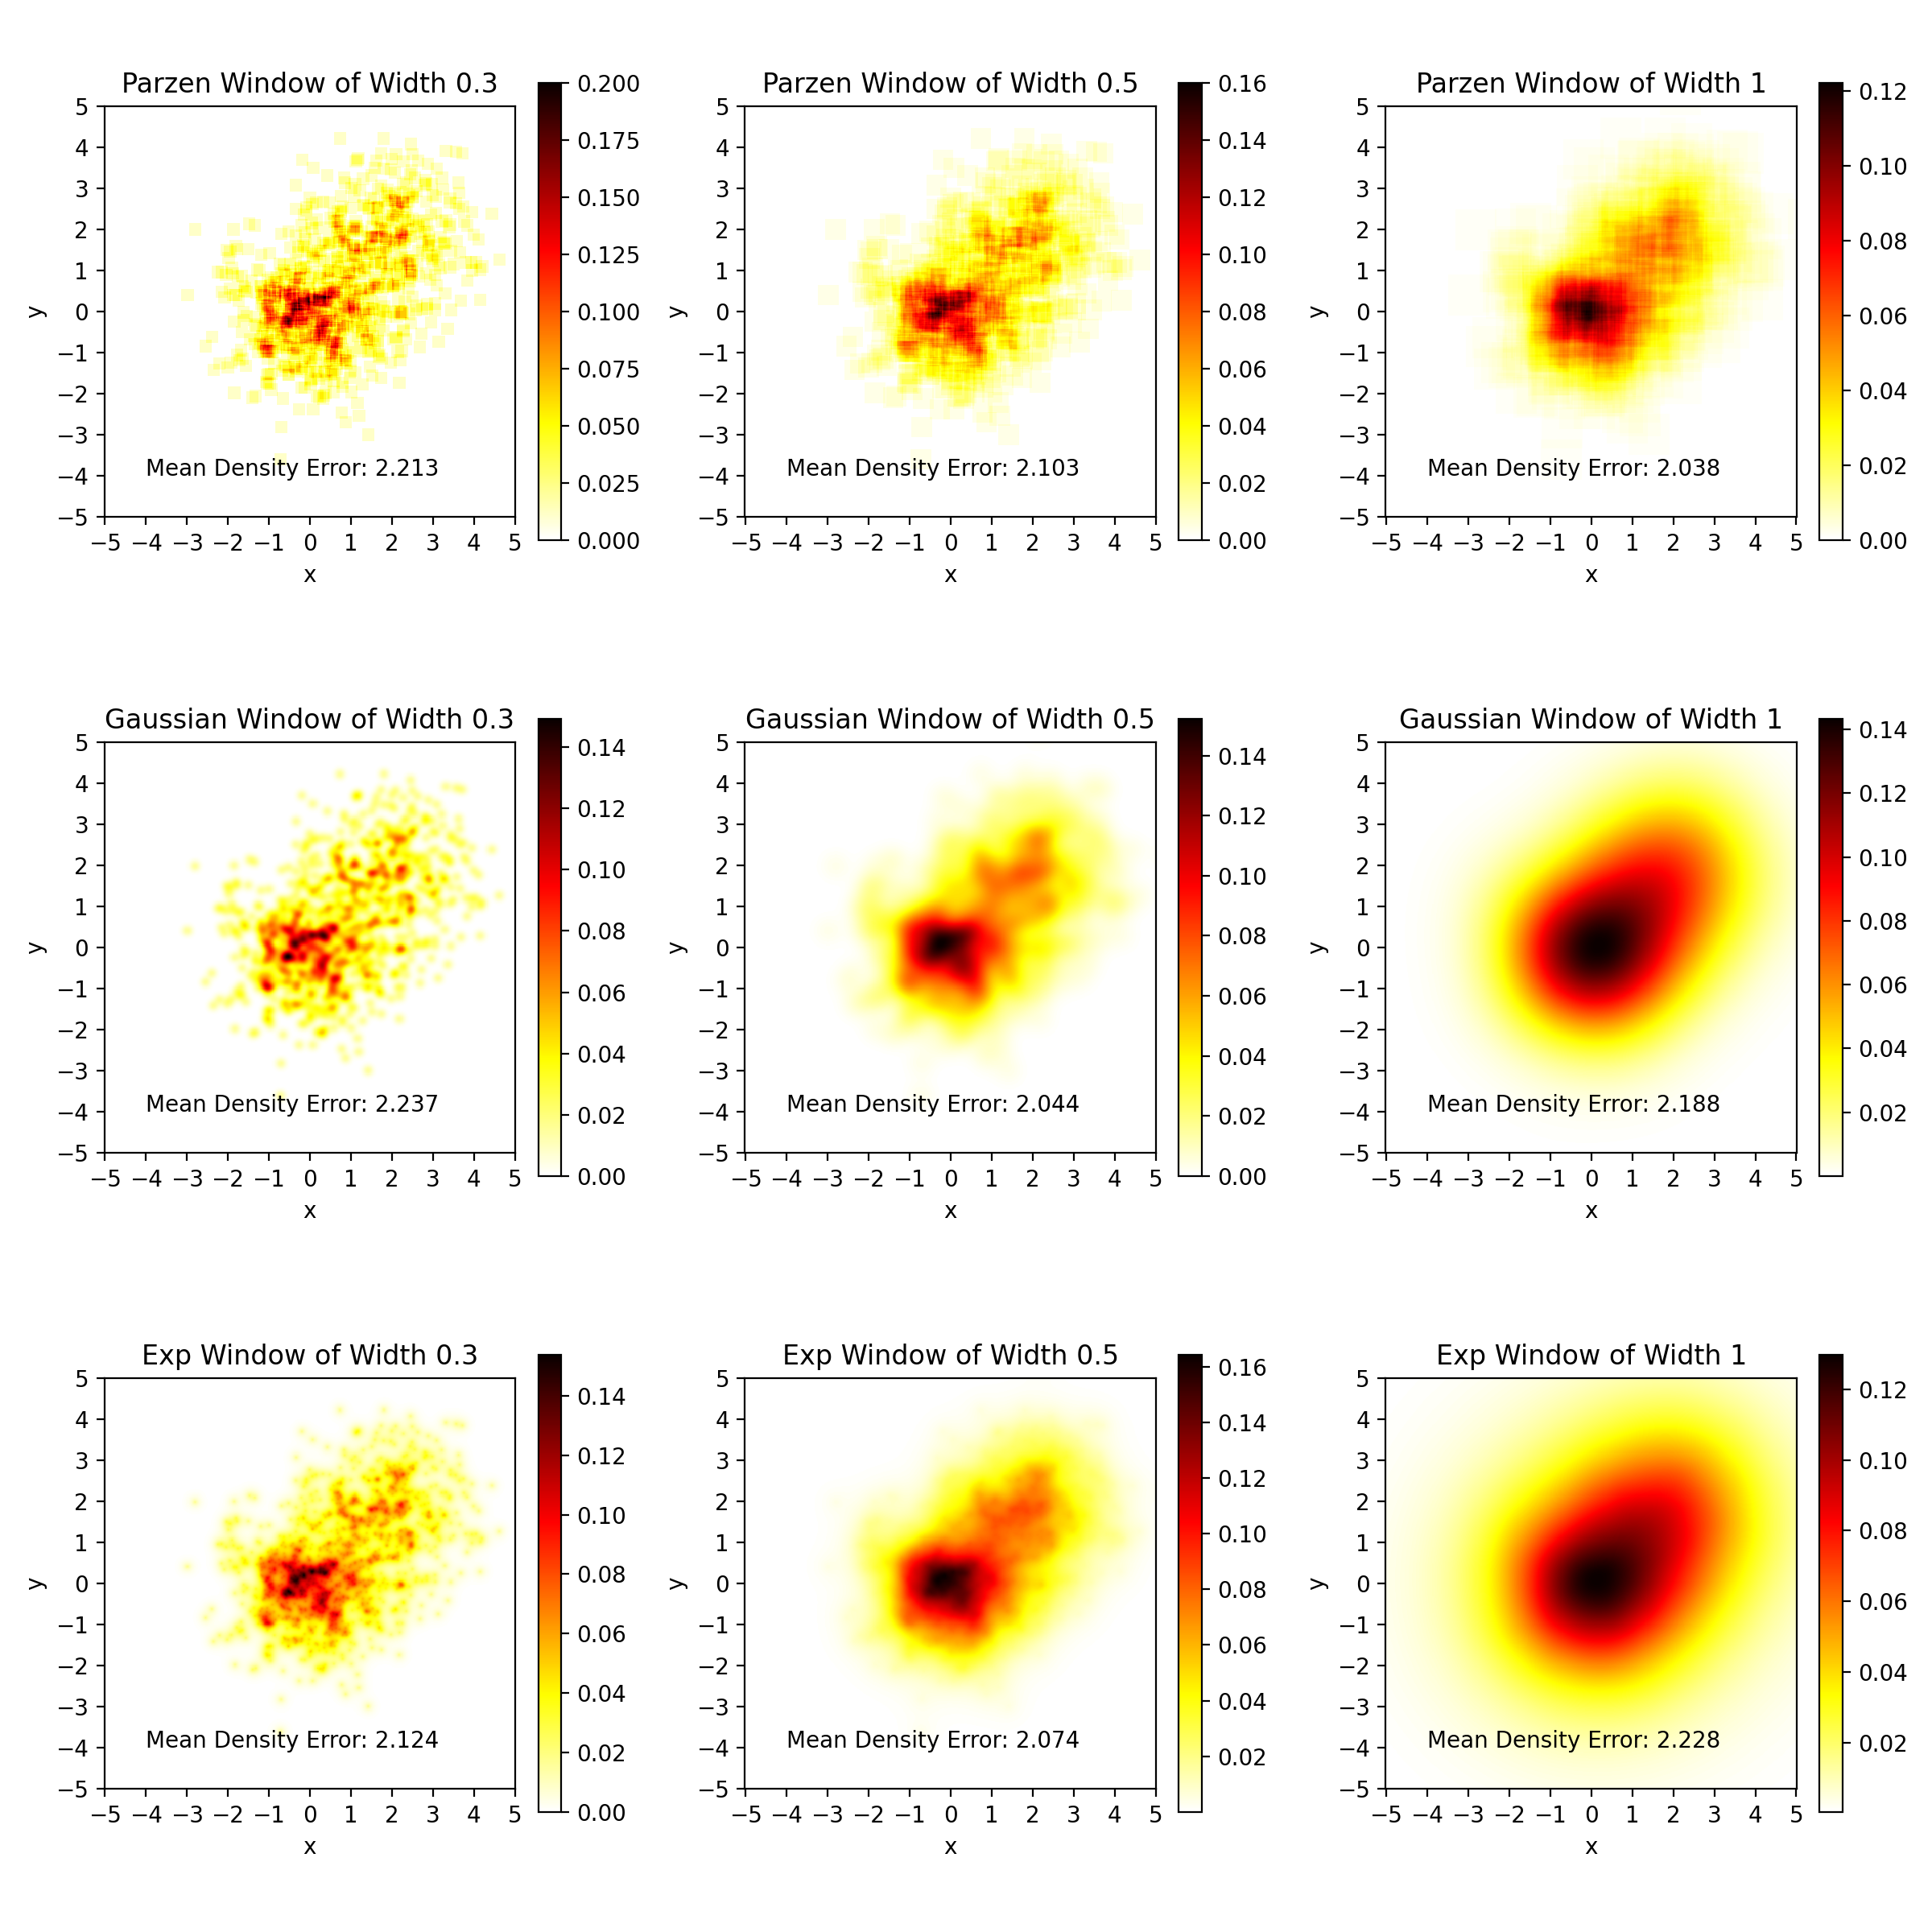
\includegraphics[width=16cm]{all.png}
  \caption{The heatmap of desity function of different kernels and window widths}
  \label{all}
\end{figure}

\end{homeworkProblem}

% \newpage
% \Acknowledgement{Thank Siying Yang 2020012981 for
% the discussion about Problem 2.3 and Problem 3.}

% End edit to here
%%%%%%%%%%%%%%%%%%%%%%%%%%%%%%%%%%%%%%%%%%%%%%%%%%%%%%%%%%%%%

\end{spacing}
\end{document}

%%%%%%%%%%%%%%%%%%%%%%%%%%%%%%%%%%%%%%%%%%%%%%%%%%%%%%%%%%%%%
